\documentclass[11pt]{article}
\usepackage[top=0.85in,bottom=0.85in,left=0.9in,right=0.9in]{geometry}
\usepackage{amsmath,amssymb}
\usepackage{graphicx}
\usepackage{booktabs}
\usepackage{enumitem}
\usepackage{xcolor}
\usepackage[colorlinks=true,linkcolor=blue!55!black,urlcolor=blue!55!black]{hyperref}
\usepackage{parskip}
\usepackage{titlesec}
\titlespacing*{\section}{0pt}{9pt}{4pt}
\titlespacing*{\subsection}{0pt}{7pt}{3pt}

\newcommand{\Sw}{S_W}
\newcommand{\Sb}{S_B}
\newcommand{\St}{S_T}
\newcommand{\rank}{\operatorname{rank}}

\title{\vspace{-1.2cm}\textbf{Eigenfaces vs.\ Fisherfaces}\\[2pt]
\large CS 740 project report}
\author{Saumya Bajpai (26D0366) \and Shubh Karman Singh (26M0843)}
\date{}

\begin{document}
\maketitle
\vspace{-1.0cm}

\section{The paper, and what we took from it}

We implement Belhumeur, Hespanha \& Kriegman, \emph{``Eigenfaces vs.\
Fisherfaces: Recognition Using Class Specific Linear Projection''}, IEEE TPAMI
19(7), 1997. Its argument is that PCA keeps the directions of largest
\emph{variance}, and under changing illumination the largest variance is the
lighting, not the identity. Fisher's linear discriminant instead keeps the
directions that separate \emph{classes}, so it discounts exactly the variation
PCA preserves.

\paragraph{What the paper contains.} Section 2 defines four methods
(correlation, eigenfaces, Linear Subspace, Fisherfaces). Section 3.1 tests
lighting on the \emph{Harvard} database (5 people, 330 images, 5 subsets by
light angle); Section 3.2 tests expression and eye wear on the \emph{original
Yale} database (16 people, 160 images) by leave-one-out; Section 3.3 is a
glasses/no-glasses test on 36 images.

\paragraph{What we implemented.} The Fisherfaces algorithm in full, plus three
of the four methods: correlation, eigenfaces (including the ``drop the first
three components'' variant) and Fisherfaces.

\paragraph{What we did \emph{not} implement.} The \textbf{Linear Subspace}
method of Section 2.3, which builds a separate 3-D illumination subspace per
person. We also did not use the paper's databases, for a practical reason: the
Harvard set comes from Hallinan's 1995 PhD thesis and has no surviving public
download, and the 1997 Yale set is a different, smaller database from the one
distributed today. We therefore used:

\begin{center}
\small
\begin{tabular}{lllp{3.3cm}}
\toprule
database & size & varies & role here \\
\midrule
ORL & $40\times10$, $92\!\times\!112$ & pose, expression, glasses & the hard case for LDA \\
CroppedYale & $38\times\!\sim\!64$, $168\!\times\!192$ & illumination only & the paper's claim \\
\bottomrule
\end{tabular}
\end{center}

CroppedYale is by the same authors (Georghiades, Belhumeur \& Kriegman, 2001)
and is the modern successor to the Harvard set, with 38 subjects rather than 5.
Our angle-binned experiment (\S\ref{sec:extra}, E5) is therefore
\emph{modelled on} the paper's Section 3.1 protocol rather than a reproduction
of it.

\paragraph{Data and code.} Code:
\href{https://github.com/qascade/eigenfaces-vs-fisherfaces}{\texttt{github.com/qascade/eigenfaces-vs-fisherfaces}}.
The databases are \emph{not} redistributed there --- Extended Yale B's terms
forbid incorporating its images into a larger publicly distributed database
without Yale's permission --- so download them from the original sources:
\href{https://www.cl.cam.ac.uk/research/dtg/attarchive/facedatabase.html}{ORL
(Cambridge Computer Laboratory)} and
\href{https://datarepo.eng.ucsd.edu/visiondata/iskwak/public_html/ExtYaleDatabase/ExtYaleB.html}{Extended
Yale B, cropped (UCSD)}. Unzip both one level above the code so \texttt{ORL/}
and \texttt{CroppedYale/} sit beside \texttt{fisherfaces\_project/}. The Yale
folders ship as \texttt{yaleB01}--\texttt{yaleB39} with \texttt{yaleB14}
absent, which is not a countable range, so \texttt{rename\_yale.sh} renames
them to \texttt{s1}--\texttt{s38} once; this changes no result, because the
class label is the loop index and never the folder name.

\section{The algorithm, and only the mathematics the code uses}

\paragraph{Notation.} $d$ pixels per image, $N$ training images, $c$ people,
$n_j$ images of person $j$, $m$ the PCA dimension used before LDA. Each image
is unrolled column-by-column into $x\in\mathbb{R}^d$ (\texttt{im(:)} in
MATLAB); $\bar{x}$ is the mean face and $X$ holds the centred training images
as columns.

\subsection{Eigenfaces, and the \texorpdfstring{$L=X^{\!\top}\!X$}{L = X'X} trick}

PCA needs the top eigenvectors of $C=\tfrac1N XX^{\!\top}$, which is
$d\times d$ --- for Yale that is $32256^2$, about 8.3\,GB, so we cannot even
store it. We do not have to. If $L=X^{\!\top}\!X$ (only $N\times N$) satisfies
$Lw=\lambda w$, multiply on the left by $X$:
\[
  X\big(X^{\!\top}\!Xw\big)=X(\lambda w)
  \quad\Longrightarrow\quad
  \big(XX^{\!\top}\big)(Xw)=\lambda\,(Xw),
\]
so $Xw$ is an eigenvector of $XX^{\!\top}$ with the \emph{same} eigenvalue.
We solve a $192\times192$ problem instead of a $10304\times10304$ one. The same
calculation gives $\|Xw\|^2=w^{\!\top}X^{\!\top}\!Xw=\lambda$, so
$\|Xw\|=\sqrt{\lambda}\neq1$ and the columns must be renormalised, otherwise
the projection is not orthogonal. (\texttt{saumya\_pca.m})

\subsection{Fisher's criterion and the two scatter matrices}

With class means $\mu_j$ and overall mean $\bar{x}$,
\[
  \Sw=\sum_{j=1}^{c}\sum_{x\in X_j}(x-\mu_j)(x-\mu_j)^{\!\top},
  \qquad
  \Sb=\sum_{j=1}^{c}n_j(\mu_j-\bar{x})(\mu_j-\bar{x})^{\!\top},
\]
and we maximise $J(w)=\dfrac{w^{\!\top}\Sb w}{w^{\!\top}\Sw w}$, whose
stationary points satisfy the generalised eigenproblem $\Sb w=\lambda\Sw w$.
Note $J$ is unchanged if $w$ is scaled, since numerator and denominator are
both quadratic --- we use this in \S\ref{sec:unitnorm}.

\subsection{Two rank bounds that decide everything}

\textbf{$\rank(\Sb)\le c-1$.} $\Sb$ is a sum of $c$ rank-one terms spanned by
the $\mu_j-\bar{x}$, and those satisfy one linear relation,
$\sum_j n_j(\mu_j-\bar{x})=N\bar{x}-N\bar{x}=0$. So $c$ vectors with a
dependence span at most $c-1$ dimensions. \textbf{Hence there are at most
$c-1$ Fisherfaces, whatever $d$ and $N$ are.}

\textbf{$\rank(\Sw)\le N-c$.} Within class $j$ the $n_j$ centred columns sum to
zero, so they span at most $n_j-1$ dimensions; summing,
$\sum_j(n_j-1)=N-c$. Read this as \emph{degrees of freedom}: each person
donates only $n_j-1$ directions. ORL with 6 images per person donates
\textbf{5}; Yale with 40 donates \textbf{39}.

\textbf{Consequence.} In pixel space $\Sw$ is $d\times d$ with rank at most
$N-c$ ($1482\ll32256$ for Yale), so it is singular and $J$ is undefined. The
paper's fix, which we follow, is to project onto $m\le N-c$ PCA directions
first. Combining the two bounds, $m$ is squeezed from both sides:
\[
  \boxed{\;c-1\;\le\;m\;\le\;N-c\;}
\]
the lower bound because $c-1$ directions cannot be extracted from fewer than
$c-1$ dimensions. We found this one by crashing the sweep in E1.

\subsection{Solving it: Cholesky whitening}

$\Sw^{-1}\Sb$ is not symmetric (its transpose is $\Sb\Sw^{-1}$), so instead we
use $\Sw=R^{\!\top}R$ (Cholesky) and substitute $w=R^{-1}z$:
\[
  \Sb R^{-1}z=\lambda R^{\!\top}RR^{-1}z=\lambda R^{\!\top}z
  \quad\xrightarrow{\ \times R^{-\top}\ }\quad
  \underbrace{R^{-\top}\Sb R^{-1}}_{M}z=\lambda z,
\]
and $M^{\!\top}=R^{-\top}\Sb^{\!\top}R^{-1}=M$, so a generalised problem has
become an ordinary \emph{symmetric} one: real eigenvalues, orthogonal
eigenvectors. Recover $w=R^{-1}z$. In code this is
\verb|M = (R')\(Sb/R)| --- two triangular solves, \emph{no inverse is ever
formed}. The paper specifies none of this; it says only ``the generalized
eigenvectors of $\Sb$ and $\Sw$'', so the solver is our choice.

\subsection{The step that is easy to miss}
\label{sec:unitnorm}

The columns returned satisfy $W^{\!\top}\Sw W=I$, i.e.\ they are
$\Sw$-orthogonal, \emph{not} Euclidean-orthogonal, so their lengths differ by
orders of magnitude. $J$ does not care, but nearest-neighbour \emph{Euclidean}
distance does. Unit-norming each Fisherface is therefore not cosmetic:
\textbf{omitting it costs ORL $90.6\%\to20.3\%$ and Yale $67.2\%\to13.5\%$} ---
same subspace, same theory, ruined classifier.

\section{Main result}

Nearest neighbour in the projected space; ORL uses 6 train / 4 test per person
over 32 people, Yale 40 train per person over 38.

\begin{center}
\small
\begin{tabular}{lcccc}
\toprule
 & correlation & eigenfaces (best $k$) & eigenfaces ($k=c-1$) & \textbf{Fisherfaces} \\
\midrule
ORL  & 91.4\% & \textbf{95.3\%} & 94.5\% & 90.6\% \\
Yale & 43.0\% & 34.2\% & 29.5\% & \textbf{67.2\%} \\
\bottomrule
\end{tabular}
\end{center}

\textbf{On Yale the paper's claim reproduces clearly}: Fisherfaces roughly
double eigenfaces, with the same number of features. Two further checks
agree with the paper: dropping the top three principal components raises Yale
from $34.2\%$ to $58.7\%$ (they encode lighting), and the same operation
\emph{hurts} ORL ($95.3\%\to87.5\%$, where they encode identity).

\textbf{On ORL Fisherfaces lose}, to eigenfaces at matched dimension
($90.6$ vs $94.5$) and even to raw-pixel correlation ($91.4$). We report this
rather than tune it away. The mechanism is the asymmetry in how the two methods
use their matrices: eigenfaces never estimates $\Sw$ and keeps the
\emph{largest} eigenvalues of a well-estimated $\St$, while Fisherfaces must
\emph{invert} $\Sw$ and so leans on its \emph{smallest} eigenvalues, which are
the worst estimated --- and ORL supplies only 5 degrees of freedom per person.
At $m=N-c$, $\operatorname{cond}(\Sw)=7.85\times10^{7}$.

Consistently, the two bases look different: eigenfaces are smooth and
face-like, Fisherfaces are high-frequency and concentrated around the eyes and
brow, because whitening scales direction $l$ by $1/\sqrt{\lambda_l}$ and so
amplifies the fine-detail directions.

\begin{figure}[htbp]
\centering
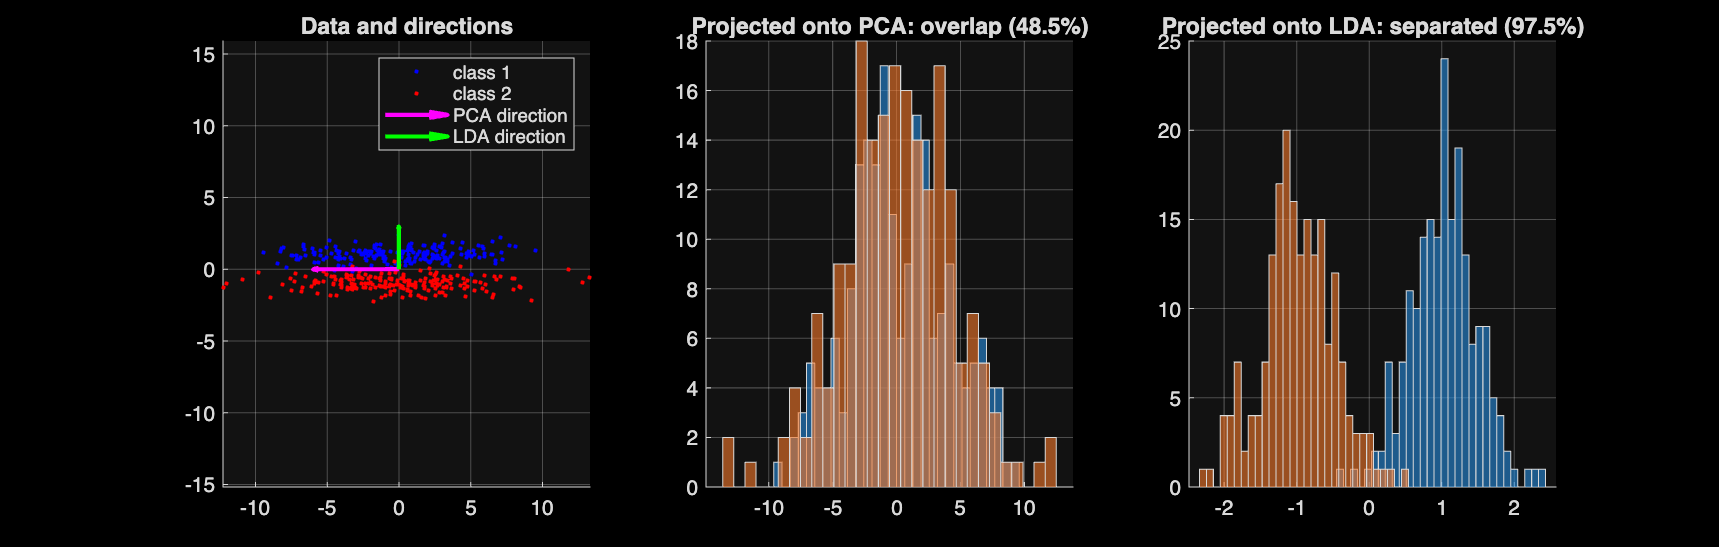
\includegraphics[width=0.49\textwidth]{figures/toy.png}
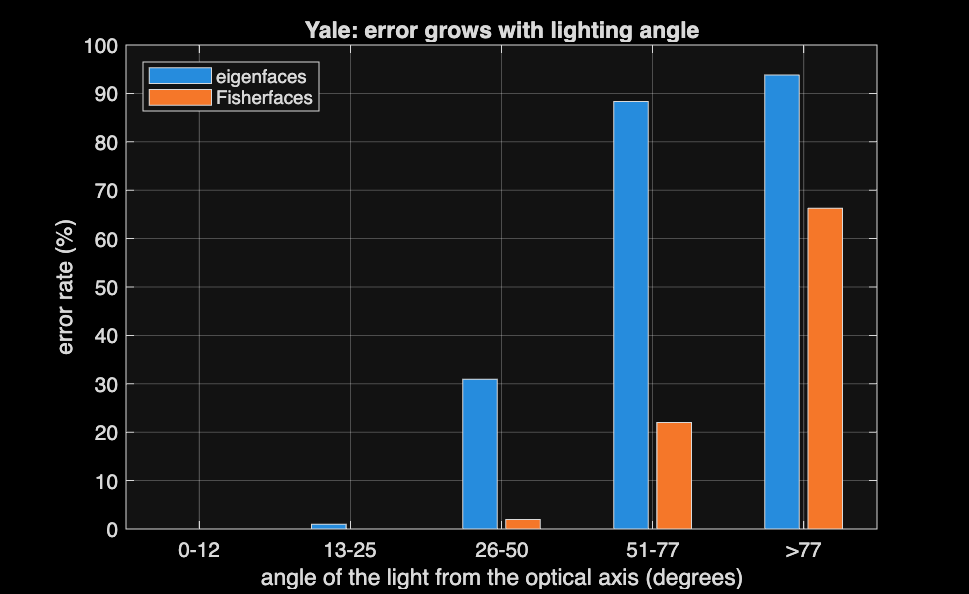
\includegraphics[width=0.49\textwidth]{figures/E5_lighting_angle.png}
\caption{Left: the 2-D toy problem. All the spread is along $x$ and all the
class information along $y$, so PCA picks the useless direction ($48.3\%$
error) and Fisher the useful one ($2.0\%$). Right: Yale error against the angle
of the light source --- the gap widens sharply as lighting becomes extreme.}
\end{figure}

\section{What we did beyond the paper, and on what data}
\label{sec:extra}

All seven run from \texttt{saumya\_experiments.m}. E1--E4 and E6 are ours; E5
is modelled on the paper's Section 3.1; E7 follows its Section 3.3.

\begin{description}[leftmargin=1.1em,style=nextline,itemsep=2pt]

\item[E1 --- $\operatorname{cond}(\Sw)$ against $m$ (ORL and Yale).]
Conditioning is flat for most of the range then turns almost vertical in the
last few steps before $m=N-c$: on Yale it grows $8.4\times10^{9}$-fold across
the sweep, and the final step $1200\to1482$ alone multiplies it by $1650$,
reaching $6.0\times10^{12}$. \textbf{The paper's $m=N-c$ is not optimal on either
database} --- ORL peaks at $m=60$ with $95.3\%$ (vs $90.6\%$), Yale at
$m=1000$ with $69.8\%$ (vs $67.2\%$). We also checked the naive
$\Sw^{-1}\Sb$ solver at every $m$: it gives identical rates and agrees with
Cholesky to $0.00^\circ$, so for this data it is not wrong --- we prefer
Cholesky for speed and guarantees, not accuracy.

\item[E2 --- Label permutation (ORL).]
Shuffling the training labels sends eigenfaces to $0.8\%$ and Fisherfaces to
$0.0\%$, against a chance rate of $3.1\%$, so the headline numbers are not a
leak. \emph{Below} chance rather than at it, because Fisherfaces faithfully
separates the shuffled grouping and is therefore systematically wrong.

\item[E3 --- Cross-validated $m$ (ORL).]
Six-fold leave-one-out inside the training set, recomputing PCA per fold,
chooses $m=40$ and scores $\mathbf{93.0\%}$; tuning $m$ on the test set would
have chosen $m=60$ for $95.3\%$. \textbf{The $2.3$-point gap is the optimism
avoided by not peeking}, and $93.0\%$ is our honest estimate.

\item[E4 --- Noise robustness (ORL), a prediction tested.]
Because Fisherfaces are higher-frequency, they should be more noise-fragile.
Our first sweep stopped at $\sigma=80$ and found nothing --- all methods moved
$0.8$ points, which on 128 test images is \emph{one image}. Extending to
$\sigma=640$ confirms it: Fisherfaces lose $60.2$ points against eigenfaces'
$21.9$. Caveat: the effect only appears far beyond realistic noise.

\item[E5 --- Error against lighting angle (Yale).]
Binning test images by $\theta=\arccos(\cos\text{az}\cdot\cos\text{el})$ read
from the filenames:

\begin{center}\small
\begin{tabular}{lccccc}
\toprule
angle & $0$--$12^\circ$ & $13$--$25^\circ$ & $26$--$50^\circ$ & $51$--$77^\circ$ & $>77^\circ$ \\
images & 0 & 104 & 152 & 300 & 338 \\
\midrule
eigenfaces  & --- & 1.0\% & 30.9\% & 88.3\% & 93.8\% \\
Fisherfaces & --- & \textbf{0.0\%} & \textbf{2.0\%} & \textbf{22.0\%} & \textbf{66.3\%} \\
\bottomrule
\end{tabular}
\end{center}

Error climbs and the gap widens --- at $26$--$50^\circ$ Fisherfaces are
$15\times$ better. The empty first bin is itself a finding (\S\ref{sec:obs}).

\item[E6 --- Sweeping the number of classes (ORL).]
For $c=2,4,8,16,32$ the number of Fisherfaces produced is
$1,3,7,15,31$ --- exactly $c-1$ every time, so the rank bound is a live
constraint, not just a proof. Fisherfaces reach $100\%$ for $c\le8$ and fall to
$90.6\%$ at $c=32$ as the problem gets harder.

\item[E7 --- Glasses / no glasses (ORL), the paper's Section 3.3.]
A different question: not \emph{who} is this, but \emph{is this person wearing
glasses}. With $c=2$ there is exactly \textbf{one} Fisherface. ORL ships no
glasses labels, so we labelled all 400 images by inspection
(\texttt{orl\_glasses\_labels.txt}; 117 wear glasses, and 8 subjects appear
both ways). We balanced the set to $50/50$ and used leave-one-\emph{subject}-out,
so the test face is never seen and identity cannot help.

\begin{center}\small
\begin{tabular}{lcc}
\toprule
method & our error & paper's error \\
\midrule
PCA, $k=10$ & 44.9\% & 52.6\% \\
one Fisherface & \textbf{41.0\%} & \textbf{5.3\%} \\
always answer ``no'' & 50.0\% & 50.0\% \\
\bottomrule
\end{tabular}
\end{center}

\textbf{We reproduce the paper's finding that PCA is near chance, but not that
Fisherfaces solve the task.} We think the difference is the data, not the
method: the paper's 36 images were \emph{paired} --- the same person
photographed with and without glasses, same session and lighting --- so glasses
were the only thing that changed. In ORL glasses co-vary with pose, expression
and session, so the single Fisher direction has no clean signal to lock onto.
This is a negative result and we report it as one.
\end{description}

\section{Observations and conclusions}
\label{sec:obs}

\begin{enumerate}[leftmargin=1.3em,itemsep=2pt]

\item \textbf{The Yale baseline was mostly a filename accident.} Lighting is
encoded as \texttt{A+020}/\texttt{A-020} and \texttt{dir} sorts as text, where
\texttt{'+'} precedes \texttt{'-'}. Taking the first 40 files therefore trains
on positive azimuths and tests on negative ones. Randomising the split roughly
doubles every method: Fisherfaces $67.2\%\to97.1\%$, eigenfaces
$34.2\%\to70.0\%$. The same accident explains E5's empty $0$--$12^\circ$ bin:
training absorbed all the frontal lighting, so every test image is at least
$12^\circ$ off axis and $638$ of $894$ are beyond $50^\circ$.

\item \textbf{\texttt{rank} and \texttt{chol} can disagree, and both be right.}
At Yale's $m=N-c$, \texttt{rank} reports $1481$ while \texttt{chol} succeeds.
\texttt{rank}'s tolerance is $\max(\text{size})\cdot\varepsilon\cdot\lambda_{\max}
=3.3\times10^{-13}\lambda_{\max}$, while $\lambda_{\min}=1.7\times10^{-13}\lambda_{\max}$
--- below one threshold, above the other. This is what ``zero slack at
$m=N-c$'' looks like in practice, and it is why we defend the solver with a
measurement rather than with ``$\Sw$ is full rank''.

\item \textbf{The rank bound appears as a cliff, not a decay.} On ORL the
generalised eigenvalues run $1.49\times10^{7}$ down to $\lambda_{31}=7.47$ and
then $\lambda_{32}=2.1\times10^{-12}$ --- twelve orders of magnitude between
consecutive eigenvalues, exactly at the predicted index.

\item \textbf{On Yale, doing nothing beats PCA.} Correlation on raw pixels
scores $43.0\%$ against eigenfaces' $34.2\%$. A sophisticated method can be
worse than no method when its objective is the wrong one.

\item \textbf{Few samples per class is not by itself what hurts ORL.} At 2
images per person on Yale --- one degree of freedom, worse than ORL's five ---
Fisherfaces still beat eigenfaces $43.0\%$ to $19.9\%$. The real account is
benefit versus cost: Yale's within-class variation is illumination, which is
huge, shared across people and nearly low-dimensional, so even one degree of
freedom finds it; ORL's is pose and expression, which is small and
idiosyncratic, so the estimation noise in $\Sw^{-1}$ dominates.

\item \textbf{Conclusion.} The paper's central claim holds and is
mechanistic, not incidental: when within-class variation is large, structured
and shared, discounting it is worth far more than the cost of estimating it,
and Fisherfaces win decisively. When it is small and idiosyncratic, the cost
dominates and plain PCA --- or even no projection at all --- is better. The
$m=N-c$ prescription is defensible but not optimal, and the honest accuracy
after choosing $m$ without touching the test set is $93.0\%$ on ORL.
\end{enumerate}

\paragraph{Code.} Three scripts, with helper functions at the bottom of each:

\begin{center}\small
\begin{tabular}{ll}
\toprule
file & what it runs \\
\midrule
\texttt{toy.m} & the 2-D toy problem of Section~2 \\
\texttt{eigenfaces\_vs\_fisherfaces.m} & the main comparison, ORL and Yale \\
\texttt{experiments.m} & experiments E1--E7 \\
\texttt{figures/} & every figure the scripts produce \\
\bottomrule
\end{tabular}
\end{center}

Every number above appears in the \texttt{run\_log} files. Full
derivations are in the accompanying study guide.

\end{document}
